\scanpage{4}
\mspage{\handwritten{(30}}
\begingroup
\reversemarginpar
\makeatletter\tagsleft@true\makeatother
\noindent\margin{\handwritten{$\varphi\qquad \varepsilon_{\xi'}$}}%
\handwritten{\tikz[baseline=-.2ex]{\draw (0,0) .. controls (.13,.16) and (.36,.24) .. (.43,.21) .. controls (.45,.19) and (.45,.17) .. (.45,.16);}}\,
Lorsque $\handwritten{\varphi}$ est de la forme $\handwritten{\varepsilon_{\xi'\raisebox{.45ex}{$\scriptstyle\deleted{\unsure{\xi'|\xi}}$}}}$, donc
\margin{\handwritten{$\varphi$}}
\[
\handwritten{\varphi} \handwritten{\simeq} \mathop{\underset{\handwritten{\longrightarrow}}{\mathrm{lim}}}\limits_j {X'_j}^{\handwritten{\unsure{\vee|v}}}\ , 
\]
on a donc une bijection naturelle
\margin{\handwritten{$\varepsilon_{\xi}\quad\varepsilon_{\xi'}\qquad .$}}
\[
\operatorname{Hom}\bigl(\handwritten{\varepsilon_{\substack{\deleted{\unsure{\xi}}\\[-.4ex]\xi}}},\handwritten{\varepsilon_{\substack{\deleted{\unsure{\xi}}\\[-.4ex]\xi\unsure{'}}}} ,\bigr)
 \handwritten{\simeq} \mathop{\underset{\handwritten{\longleftarrow}}{\mathrm{lim}}}\limits_i \mathop{\underset{\handwritten{\longrightarrow}}{\mathrm{lim}}}\limits_j \operatorname{Hom}_{X}(X'_j,X_i)\handwritten{\deleted{\unsure{,|.}}}\qquad .
\tag*{$(*)$}
\]

\noindent D'autre part on a (dans la catégorie des préschémas)
\margin{\handwritten{$\deleted{\unsure{\xi}}$}}
\[
\bar X(\handwritten{\xi}) == \mathop{\underset{\handwritten{\longleftarrow}}{\mathrm{lim}}}\limits_i X_i\handwritten{\deleted{\xi}}\ ,\quad
\bar X(\handwritten{\xi}') = \mathop{\underset{\handwritten{\longleftarrow}}{\mathrm{lim}}}\limits_j X'_j\ ,
\]
d'où
\[
\handwritten{\tikz[baseline=-.2ex]{\draw (0,0) .. controls (.08,-.03) and (.18,.03) .. (.23,.08);}}\; \operatorname{Hom}_{X}(\bar X(\handwritten{\xi}'),\bar X(\handwritten{\xi})) \handwritten{\simeq}
 \mathop{\underset{\handwritten{\longleftarrow}}{\mathrm{lim}}}\limits_i \operatorname{Hom}_{X}(\bar X(\handwritten{\xi}'),X_i)\ ,
\]
\margin{\handwritten{\tikz{\draw (0,0) .. controls (.04,.18) and (.27,.10) .. (.49,.28) .. controls (.58,.35) and (.56,.45) .. (.54,.47);}}}
d'autre part, comme $X_i$ est loc\inserted{\handwritten{\tikz[baseline=(w.base)]{%
\node[anchor=base west,rotate=14,inner sep=.3pt] (w) at (0,0) {alement};
\draw (-.04,-.17) .. controls (-.01,.08) and (.42,.04) .. (.85,.27) .. controls (.98,.34) and (1.04,.41) .. (.99,.42);
}}} de présentation finie sur $X$\handwritten{, on a}
\[
\operatorname{Hom}_{\handwritten{X}}(\bar X(\handwritten{\xi}'),X_i) \handwritten{\simeq}
 \mathop{\underset{\handwritten{\longrightarrow}}{\mathrm{lim}}}\limits_j \operatorname{Hom}_{X}(X_j,X_i)\handwritten{,}
\]
d'où
\[
\operatorname{Hom}_{X}(\bar X(\handwritten{\xi}'),\bar X(\handwritten{\xi})) \handwritten{\simeq}
 \mathop{\underset{\handwritten{\longleftarrow}}{\mathrm{lim}}}\limits_i \mathop{\underset{\handwritten{\longrightarrow}}{\mathrm{lim}}}\limits_j \operatorname{Hom}_{X}(X'_j,X_i)\ .
\tag*{$(**)$}
\]

\noindent La comparaison de $(*)$ est $(**)$ donne la\handwritten{$\mid$}conclusion voulue (moyennant une verification de compatibilités, laissé\deleted{\unsure{n|e|s}}e au lecteur).

% slanted
\noindent\margin{\handwritten{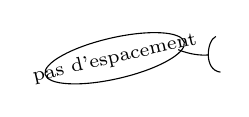
\begin{tikzpicture}[baseline,scale=.84]
\node[rotate=13,inner sep=1pt] (m) at (0,0) {\scriptsize\unsure{pas} d'espacement};
\draw[rotate=13] (0,0) ellipse [x radius=1.08cm,y radius=.31cm];
\draw (.96,.13) .. controls (1.13,.06) and (1.29,.04) .. (1.42,.05);
\draw (1.53,.33) .. controls (1.39,.27) and (1.34,-.18) .. (1.60,-.21);
\end{tikzpicture}}}%
b) \uline{Le foncteur envisagé est essentiellement surjectif:}

\noindent 7.9.1.\quad Remarquons d'abord que si $C$ est un site où les $\mathop{\underset{\handwritten{\longleftarrow}}{\mathrm{lim}}}\limits$ finies sont représentable, $\handwritten{\widetilde}{C} = \underline{E}$ le topos correspondant alors\handwritten{,} tou\deleted{s}\handwritten{t}%
\margin{\handwritten{,\quad t}}
foncteur\deleted{s} fibre\deleted{s} $\handwritten{\overset{\deleted{\unsure{\varphi|\xi}}}{\varphi}}$ sur $\underline E$ peut se représenter comme une ``limite''
\margin{\handwritten{$/\quad /\quad\varphi$}}
inductive pseudo-filtrante connex\deleted{\unsure{e}}\handwritten{e}\handwritten{''} d\deleted{e}\handwritten{e} foncteurs de la forme
\margin{\handwritten{e\quad e}}
\margin{\handwritten{$]\,[ $}}
\[
\handwritten{\check}{Y}(F) == F(Y) = \operatorname{Hom}(\handwritten{\widetilde}{Y},F),\handwritten{\big]\big[}\, Y\handwritten{\in}\operatorname{Ob} C\handwritten{,}
\]
(ou $\handwritten{\widetilde}{Y}$ est le faisceau associé à $Y$)\handwritten{,} de la façon suivante. On considèr\deleted{\unsure{e|s}}\handwritten{e}
\margin{\handwritten{,}}
la catégorie\handwritten{$\mid C_{\substack{\deleted{\unsure{\xi|\varphi}}\\[-.4ex]\varphi}}$} des couples $(Y,\handwritten{\xi})$, avec $Y\handwritten{\in}\operatorname{Ob} C$, $\handwritten{\xi}\handwritten{\in\varphi}(\handwritten{\widetilde}{Y})$
\margin{\handwritten{$C_{\varphi}$}}
\endgroup

% archive sheet number: 3
\clearpage
